\chapter{Introduction}
% TODO references for these
Cellular Automata (CA) are a very simple model of computation.
There are many variations and extensions of them,
and some like Conway's Game of Life and Rule 110 are known to be Turing Complete.
Isabelle is a proof assistant that can be used for anything from mathematical proofs to formal verification of software properties.

\section{Topic addressed in this project}

This project looks at formalising models of Cellular Automaton in Isabelle to help deal with the complexity that comes with trying to mathematically prove results about them.
In addition to providing a definition of six different variants of CA,
this project provides definitions of important properties they may have, and proves some lemmas and theorems necessary to work with them.

\section{Motivation}

It is very difficult to work with high level concepts while still being rigorous,
and theoretical Computer Science is a very abstract and mathematical discipline that requires exactly that.

as it strikes a balance between simplicity and complexity.
They are


\section{Approach}

\docs{Isabelle} was chosen as the language to implement these models in.

\section{Metrics}





%\begin{figure}[h]
%    \centering
%    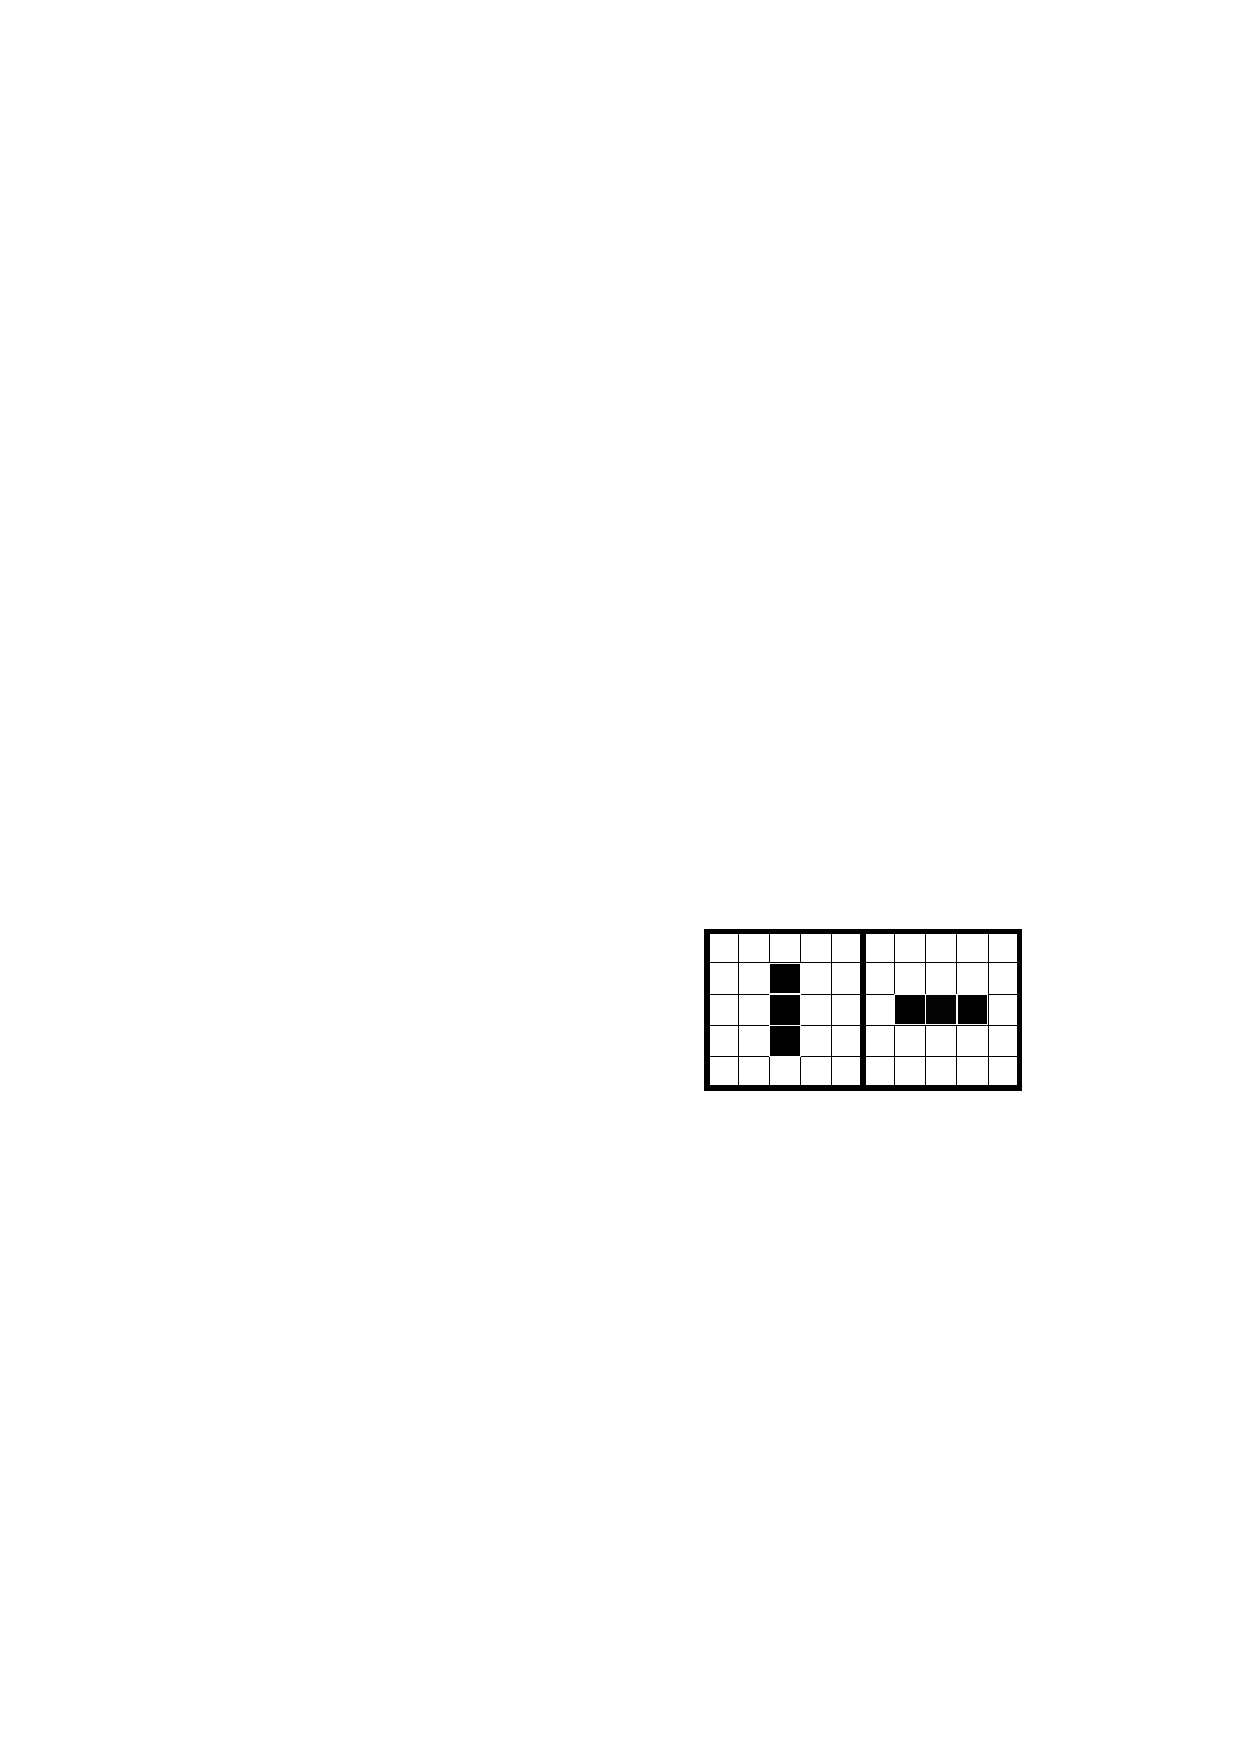
\includegraphics[scale=0.7]{blinkers_both.pdf}
%    \caption{Both forms of a Blinker}
%    \label{fig:binkers}
%\end{figure}

%\begin{myminted}{Some Example Isabelle}{testcode}
%    fun garden_of_eden :: "CA ==> bool" where
%    "garden_of_eden (CA s r) = (¬(EX s0. (CA s0 r) yields s))"
%
%    theorem "ca yields State (run ca 1)"
%    proof-
%      show ?thesis using yields_def by blast
%    qed
%\end{myminted}
